%%%%%%%%%%%%%%%%%%%%%%%%%%%%%%%%%%%%%%%%%%%%%%%%%%%%%%%%%%%%%%%%%%%%%%%%%%%%%%%%
%2345678901234567890123456789012345678901234567890123456789012345678901234567890
%        1         2         3         4         5         6         7         8

\documentclass[letterpaper, 10 pt, conference]{ieeeconf}  % Comment this line out
                                                          % if you need a4paper
%\documentclass[a4paper, 10pt, conference]{ieeeconf}      % Use this line for a4
                                                          % paper

\IEEEoverridecommandlockouts                              % This command is only
                                                          % needed if you want to
                                                          % use the \thanks command
\overrideIEEEmargins
% See the \addtolength command later in the file to balance the column lengths
% on the last page of the document



% The following packages can be found on http:\\www.ctan.org
\usepackage{graphics} % for pdf, bitmapped graphics files
\usepackage{epsfig} % for postscript graphics files
\usepackage{cite}
\usepackage{mathptmx} % assumes new font selection scheme installed
\usepackage{times} % assumes new font selection scheme installed
\usepackage{amsmath} % assumes amsmath package installed
\usepackage{amssymb}  % assumes amsmath package installed
\usepackage{pbox}
\usepackage{color, colortbl} % define new colors and the latter to actually color the table:
\usepackage{multirow}

\title{\LARGE \bf
On the origin of creatures: The evolution of virtual creatures in a rigid-body engine
}


\author{Benjamin Ellenberger% <-this % stops a space
\thanks{This research was funded by my own freetime, motivation and ideas.}% <-this % stops a space
\thanks{B. Ellenberger is with the Department of Neuroinformatics, University of Zurich, 8050, Zurich, Switzerland, email:
        {\tt\small  ellenbeb@student.ethz.ch}}%
}


\begin{document}



\maketitle
\thispagestyle{empty}
\pagestyle{empty}


%%%%%%%%%%%%%%%%%%%%%%%%%%%%%%%%%%%%%%%%%%%%%%%%%%%%%%%%%%%%%%%%%%%%%%%%%%%%%%%%
\begin{abstract}


The behavior of animals and humans is a complex combination of information processing and learning, decision making and sensory-motor interaction with the environment. The information processing and learning are strongly coupled with the motor actions, however it is not yet well understood how these segments are related in the animal brain.
\\
In this project we show how to evolve the controlling neural structure and morphology including muscular structure and sensory implementation of a population of virtual creatures in a simulated three-dimensional, physically realistic world using genetic algorithms. Creatures are created from cuboid bounding-boxes connected using one of several joint models out of the possible 3 DOF joint set and the Hill-model for the muscle simulation and are controlled by simultaneously evolved neuronal network controllers. Further it is shown how to evaluate the creature with several fitness functions and to let the creature improve its performance via Hebbian learning (Oja's rule) to pick up correlations between the different signal channels.

\end{abstract}


%%%%%%%%%%%%%%%%%%%%%%%%%%%%%%%%%%%%%%%%%%%%%%%%%%%%%%%%%%%%%%%%%%%%%%%%%%%%%%%%
\section{INTRODUCTION}
Human creativity and intelligence are two of the main components that led mankind to its technological success and helped it to become world's dominant mammal that can reach nearly any spot on earth and made a subset of it housable for its own species. The problems of today are sometimes very complex and can often not be solved by a simple, one-for-all solution. Today researchers normally have to work on solutions for many years. Some problems could never have been solved without the aid of a computer. But still it seems that the problems can not be solved by a computer alone and crucially need human creativity. To find solutions to those problems, large, multi-dimensional search spaces have to be searched for possible solutions, which is what humans are very good at and do intuitively when searching for solutions. Unfortunately, this process of research is very time-consuming, tiring and challenging and does not necessarily lead to a solution to the problem. A big issue of humans is also that the ability to think outside of the box and come up with a new, unique solution is limited by so called designer biases \cite{Pfeifer2006}. Designer biases are ideas and intuitions of the human mind with constrain the search space by giving the human mind the idea that a certain problem can be solved in a to the brain most intuitive way. This can be shown in the problem of two perpendicular water-tubes that will be connected by the human with a simple slope whereas the most efficient solution would also have to consider the direction of the flow of the water. Such issues can be tackled partly with computer aided design, which let the human define the proper constraints for the solution and the computer then helps to find the possible solutions, but the true solution to resolve this issue would be if the computer could come up with possible solutions to the problem by itself. One such self-developing approach to find optimal solutions is by artificial evolution.

An increasing number of researchers were drawn to the topic of artificial evolution after the both simple and revolutionary paper of Karl Sims had been published in 1994 \cite{Sims1994}. The fact that 3D world computer simulations were very demanding even with high performance devices prohibited the simulation of large scale 3D worlds. In the 1990s the performance of computational devices increased every year according to Moore's Law \cite{Moore1965}, but those devices were still very limited in their capabilities compared to today's personal computer device containing dedicated hardware for Graphics and Physics computations. Also the software of the time was not very mature yet and most researchers had to implement the whole framework of their simulations by themselves, which reduced either the complexity of the approaches or took a long time or a larger research group that worked on the problem. That is what makes Karl Sims papers so interesting, namely that he implemented his own rigid body physics engine and several laws of physics as the constraints to the evolutionary system as well as his own evolutionary framework which developed creatures.

\section{METHODS}

This section describes the methods of virtual creature evolution. A simulation in artificial evolution is not written from scratch, because it is just a waste of time to implement when up to today game and simulation engines have arised that simulate approximately perfect 3D rigid body physics. The only important fact about the implementation of physics for artificial evolution is that the engine under no circumstances should allow energy leaks from non-conservation, or even round-off errors, because the evolving creatures will inevitably discover and exploit them for their own purpose. Genetic algorithms are known for their high ability to exploit the smallest exploitable niches if they lead to an increase of efficiency and that is why one has to be careful in choosing what should be exploitable or not. Otherwise the results might be biased by the unfortunate exploit.
\subsection{Overview}

The simulation is written in a rigid body physics engine named bullet physics engine. This decision was taken because bullet physics is already used in various simulations and provides a framework to simulate Rigid body and soft bodies with discrete and continuous collision detection providing a rich set of rigid body and soft body constraints with constraint limits and motors \cite{bulletPhysics}. Further used was an engine called jMonkey engine which helps with the fast use of OpenGL in Java to show the graphics of the simulated creatures on screen \cite{jMonkeyEngine}. The parts of interest such as the evolutionary framework providing classes for genotypes and phenotypes, methods to mutate genes and cross-over genomes as well as the transcription, the fitness function evaluation, the sensors, the control structure including the neural network and muscle actuation were written from scratch without the use of any framework.

\subsection{Genetic language}
The genetic language to express the morphology and neuronal network configuration uses a directed cyclic graph representing genes and their interconnection. The genes are primitives for the morphological cuboids, joints and muscles, out of which the body is built, the neurons, the proprioceptive and exteroceptive sensors and the effectors.
The genome can therefore define an infinite number of individual creatures in the highly dimensional search space showing an infinite number of possible behaviors. By evolving and evaluating over generations, several successful behavior strategies can be found to perform well towards the goal that is measured by the fitness function.

\subsection{Neuronal network}
The neurons have multiple mathematical function primitives to speed up evolution as well as the biologicially inspired sum-threshold function. In the case of the sum-threshold function, Hebbian Learning to optimize the performance via the Oja's learning rule is used to see if the neuronal network can improve the performance. 

One of the earliest rules known to pick up correlations in the brain was stated by D. Hebb in his book 'The Organization of Behavior'. The Hebbian theory describes how neurons might connect to each other to become engrams, which are means to store memory traces inside of the brain as described by Richard Semon. Hebb's theories on the form and function of cell assemblies can be understood from the following: "The general idea is an old one, that any two cells or systems of cells that are repeatedly active at the same time will tend to become 'associated', so that activity in one facilitates activity in the other." \cite{Hebb1949}(p.70). "When one cell repeatedly assists in firing another, the axon of the first cell develops synaptic knobs (or enlarges them if they already exist) in contact with the soma of the second cell." \cite{Hebb1949}(p.63). The Hebb's postulate is often simplified to the conceptual terms that ''neurons that fire together, wire together''. In component form as a difference equation, it is written as:
\begin{align*}
\Delta\mathbf{w} ~ = ~ \eta\, y(\mathbf{x}_n) \mathbf{x}_{n}
\end{align*}
or in scalar form with implicit  $n$-dependence,
\begin{align*}
w_{i}(n+1) ~ = ~ w_{i} + \eta\, y(\mathbf{x}) x_{i}
\end{align*}

where $y(x_n)$ is again the output, this time explicitly dependent on its input vector $x$.

A problem with Hebb's rul is that the synaptic weights approach infinity with a positive learning rate. This can be prohibited by a normalization of the weights so that each weight's range is constrained between 0 meaning no connection and 1 meaning that the neuron is the only input neuron. This is done by normalizing the vector to length one:

\begin{align*}
w_i (n+1) ~ = ~ \frac{w_i + \eta\, y(\mathbf{x}) x_i}{\left(\sum_{j=1}^m [w_j + \eta\, y(\mathbf{x}) x_j]^p \right)^{1/p}}
\end{align*}

In Oja's original paper\cite{Oja1982}, this is done by the root sum of squares which is the familiar cartesian normalization rule. It can however by normalized with any normalization rule without loss of generality.

The neuronal network connects the exteroceptive and proprioceptive sensors with the muscles in case they are not directly connected and compute the function encapsulation defined by the connections and weights. In most cases, the calculations might not be very reasonable, but based on the primitives it is definitely possible that a useful network arises that controls the creature to succeed in the fitness evaluation.
\subsection{Fitness evaluation}
The fitness evaluation allows different fitness evaluation functions to be evaluated simultaneously and be combined to one rating via linear weighting.
The idea behind this is to be able to evaluate several fitness functions at the same time so that one can easily write another fitness function for an additional constraint. This can for instance be used to evaluate a primary goal and additionally an auxiliary fitness function measuring the existence of so called design principles for intelligent systems within the design of the creature. Further it is possible to evolve creatures for a certain task with the auxiliary fitness function. What counts for the laws of physics also counts for the fitness functions. If there is an alternative option in which the fitness function can be exploited than by the original intention, some creatures will definitely do this, especially when it is easier to exploit it this way than the intended way.
\subsection{Evolution}
The evolutionary algorithm is built upon two main ideas. The first is the evaluation step performed on one creature after another to evaluate the fitness. The second idea is then to drop the worst performing creatures of the population and replace them with offsprings of the best performing creatures. In the simulation, an instance called the reaper sorts the creatures by their performance ratings, then reaps the worst creatures and then sows new ones. The creatures are sown according to the percentages defined by the user. The user defines how many new creatures are built by crossing over the best creatures then the genes and their connections are mutated. Other percentages define how many creatures are just create from the same best performing set but the genome is only mutated and not crossed over. The best performing creatures stay part of the population to see if their offspring top them in the next run. If the population is not yet completely full again, the remaining creatures are generated randomly in the same manner as the creatures were created when the population was initialized.

\section{SIMULATIONS}
To show the abilities of the framework, two simulations were run and the results are discussed below. The first simulation was run with the fitness function measuring the speed of motion of the creature on land. Therefore it was not important how the creature achieved the locomotion and how big the creature evolved to be faster just to have a higher stride length etc.

\section{Results}

\subsection{Velocity as the fitness function}

In the first simulation, the results initially were strongly biased by the fact that there was the possibility to exploit the constraining laws of physics in another way than expected. Expected by the author was actually that the creature, instead of trying to run or roll as fast as possible, would exploit the fact that the velocity was measured by looking at the displacement of the morphological root. The morphological root is the first limb created in the phenotype of the creature. If the morphological root would be made very small and thereby very light and would be connected to a larger, heavier limb via a joint, the fitness function would be easily exploitable by swinging around the root in the air, which could easily reach a high velocity because of its weight. This setting would not move at all, but would reach a high fitness value. Instead the population found another possibility. The limb dimensions were randomly defined between 0 and a certain maximum value, which gave it the opportunity to remain very thin. With very thin, approximately zero cuboids, the collision detection fails and the creature falls through the terrain. Since the gravitational force is pulling it down, the creature accelerates with the evaluation time faster than it could ever do it by using legs on the terrain. This exploitation was chosen by about 40\% of the individuals after three generations and because of the efficiency of the strategy, all creatures took it over until the 30th generation. It can also be seen that the creatures tried to remain small as their genome size shrank from an initial average size of 160 to an average size of 80. The complete graph can be seen in figure \ref{velocity1}.

\begin{figure}[tp]
    \centering
%\hspace{-0.5ex}
    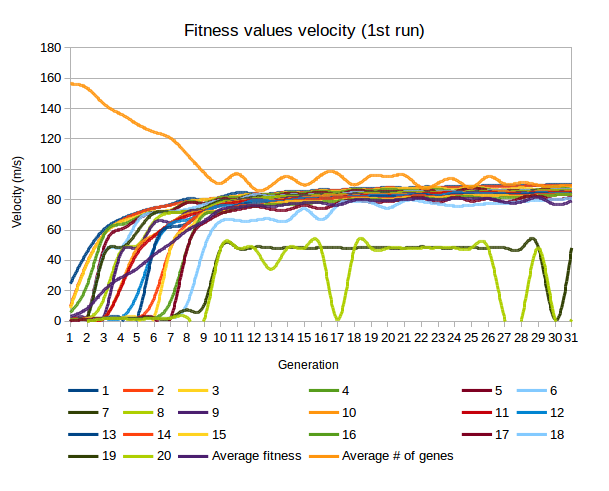
\includegraphics[width=3.4in, clip] {figs/velocity1.png}
    \caption{First run of the velocity experiments. It can be seen in the graph that the 20 individuals are taking over the gravity exploting strategy instead of trying to perform locomotion. In orange the average number of genes in the genomes can be seen as it is decreasing to reduce the size of the creatures.}
    \label{velocity1}
\end{figure}

In the second run, this behavior was suppressed by adding a minimum size for the limb dimensions instead of 0. It is therefore not possible anymore to fall through the terrain. The task's difficulty seems to have strongly increased. This can be seen as no creature achieves any type of locomotion up to generation 24. There a new individual comes into play that achieves locomotion with a spinning or propelling movement using a joint as the rotation axis. This movement is then taken over by offsprings of this individual which can perform a similar movement. The graph of the second run is shown in figure \ref{velocity2}. The creature reaching a high velocity can be seen in figure \ref{velocity-creature}.

\begin{figure}[tp]
    \centering
%\hspace{-0.5ex}
    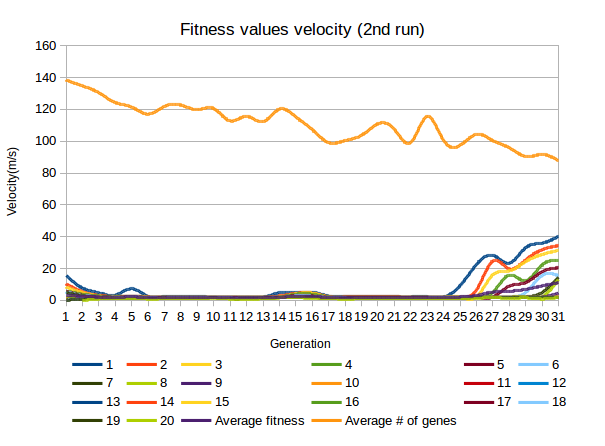
\includegraphics[width=3.4in, clip] {figs/velocity2.png}
    \caption{Second run of the velocity experiments. The task is now a harder optimization task and can not be easily exploited. Up to the generation 24 no individual is able to move in a really fast manner (< 5 $\frac{m}{s}$). After that, a new individual comes into play that uses a certain propelling movement using one of its limbs similar to a wheel or rudder.}
    \label{velocity2}
\end{figure}

\begin{figure}[tp]
    \centering
%\hspace{-0.5ex}
    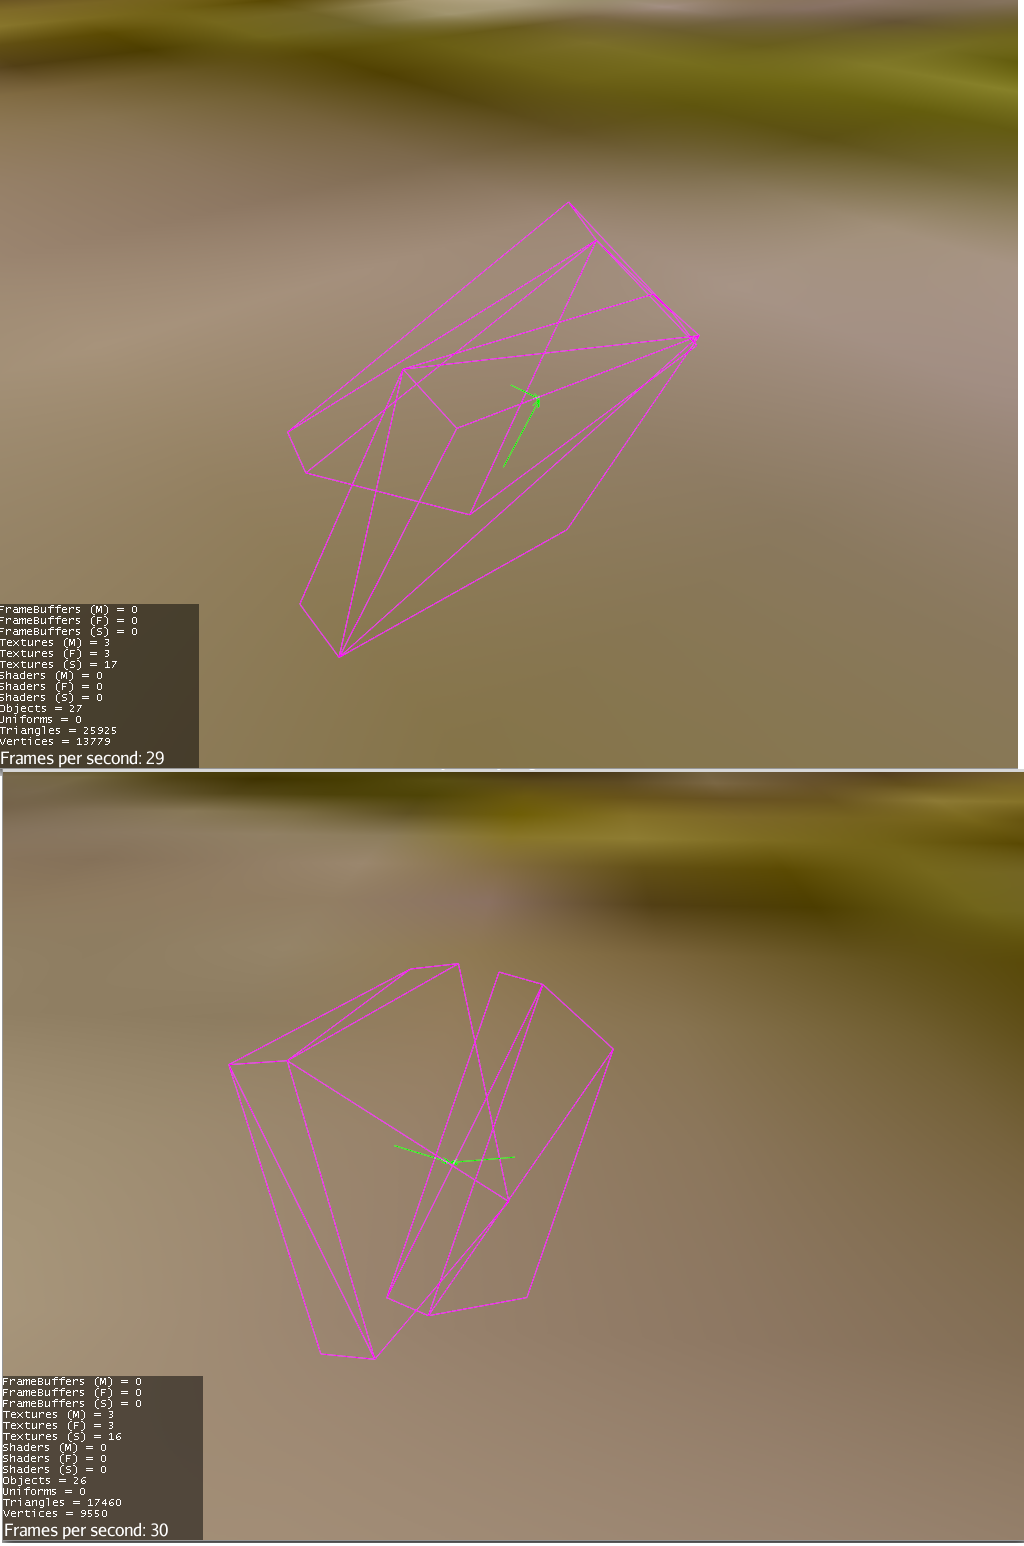
\includegraphics[width=3in, clip] {figs/velocity-creature.png}
    \caption{The new individual using a certain propelling movement using one of its limbs similar to a wheel or rudder.}
    \label{velocity-creature}
\end{figure}

\section{OUTLOOK}
Since the programming and debugging of the framework took the highest amount of time it would be a good opportunity to further improve it and implement several fitness functions into it and evaluate the effect of different numbers of cross-over partners (elitarism) and overall population size. An interesting fitness function could be the information theoretical measure called transfer entropy, originally introduced to measure the magnitude and the direction of information flow from one element to another and has been used to analyze information flows in real time series data from neuroscience, robotics, and many other fields. This could be used to verify the hypothesis that stronger information flows indicate a more coordinated behavior of the creature and a higher ability to learn new tasks \cite{Schmidt2013}. Other possibilities would be to work on real concurrency between the creatures and extend the framework to look if creatures can feed themselves from common nutrition sources and can show their dominance over the other creatures. The fitness functions in that case would be replaced by not having enough resources for all creatures so that only the successful ones can survive because of the desired features they have. It could also be shown that heritage is not helpful to one's offspring because they are not forced to compete with others if they for example inherit the energy level from their ancestors so that they can live from that energy for a longer period without food. Also the use of parallel evaluation could shorten the evaluation process, giving the researcher the opportunity to evaluate populations on high performance clusters.



\addtolength{\textheight}{-12cm}   % This command serves to balance the column lengths
                                  % on the last page of the document manually. It shortens
                                  % the textheight of the last page by a suitable amount.
                                  % This command does not take effect until the next page
                                  % so it should come on the page before the last. Make
                                  % sure that you do not shorten the textheight too much.

%%%%%%%%%%%%%%%%%%%%%%%%%%%%%%%%%%%%%%%%%%%%%%%%%%%%%%%%%%%%%%%%%%%%%%%%%%%%%%%%



%%%%%%%%%%%%%%%%%%%%%%%%%%%%%%%%%%%%%%%%%%%%%%%%%%%%%%%%%%%%%%%%%%%%%%%%%%%%%%%%


%%%%%%%%%%%%%%%%%%%%%%%%%%%%%%%%%%%%%%%%%%%%%%%%%%%%%%%%%%%%%%%%%%%%%%%%%%%%%%%%

\bibliographystyle{IEEEtran}
\bibliography{Creatures}


\end{document}
